\label{section:introduction}
%%%%%%%%%%%%%%%%%%%%%%%%%%%%%%
This manual provides a short description of the \fitter\ program 
which can be used to determine unpolarised proton parton density functions 
(PDFs). 
%using deep inelastic scattering (DIS) data and other processes such as 
%Drell-Yan, jet or ttbar processes.
The parton density functions are needed to calculate cross sections
for $ep$, $pp$, and $p\overline{p}$ colliders and thus they are required for interpetation
of the data collected at the LHC.

A schematic structure of the \fitter\ is illustrated in Fig.~\ref{fig:flow} which encapsulates all the current functionality of the platform.
\begin{figure}
\begin{center}
\caption{Schematic Structure of the \fitter\ program}
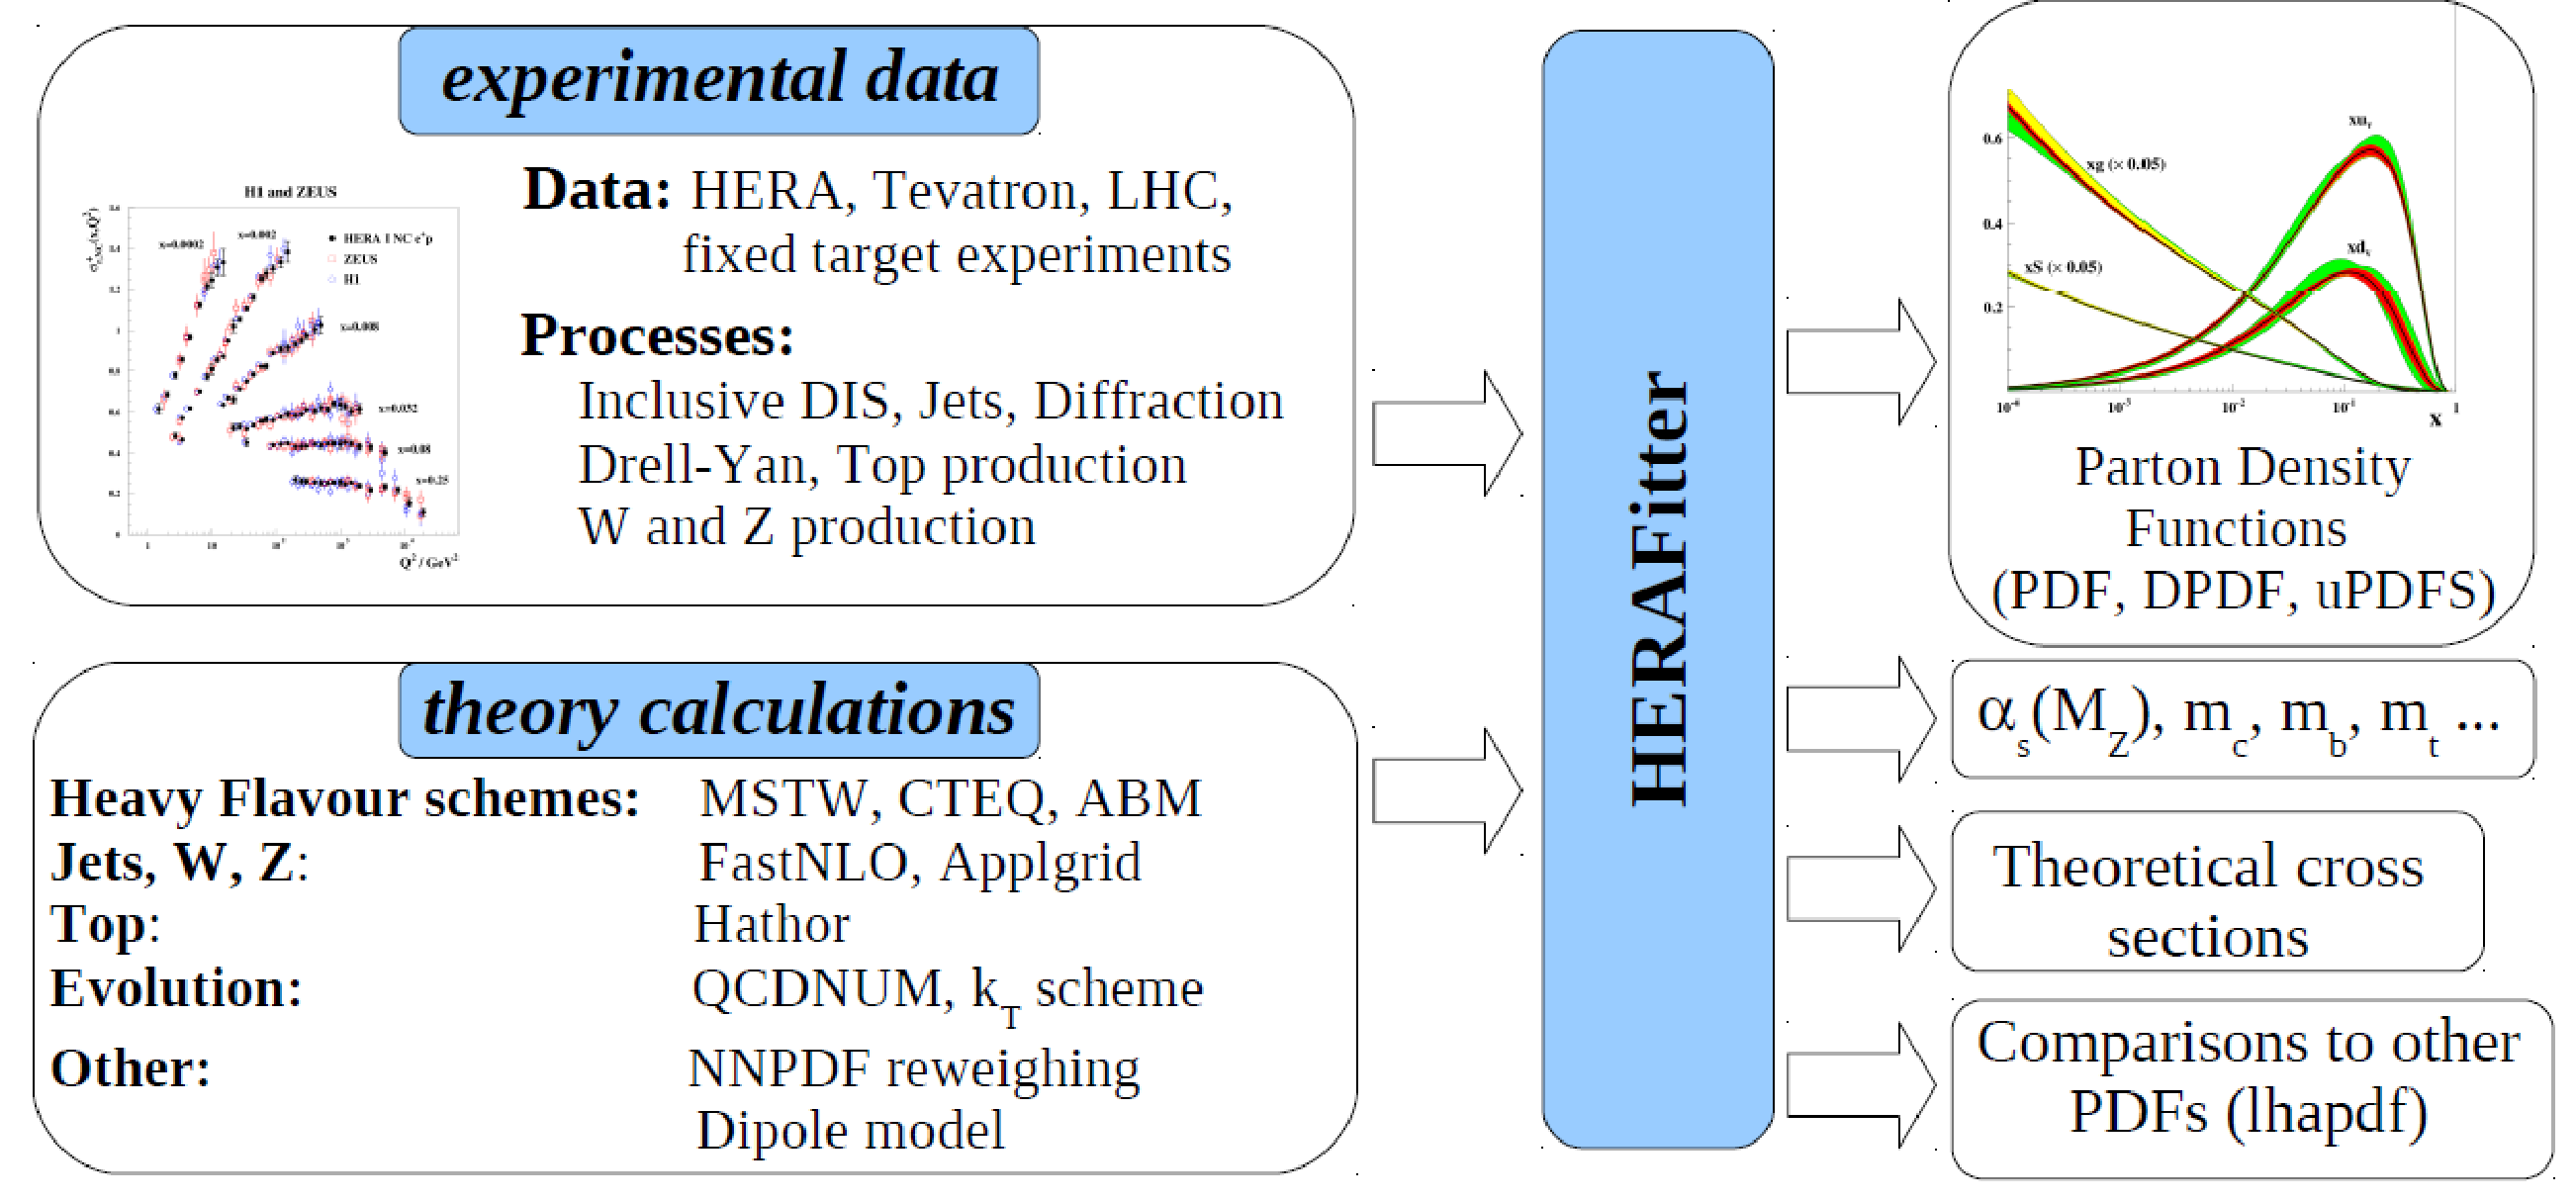
\includegraphics[width=0.75\linewidth]{figures/flow.pdf}
\end{center}
\label{fig:flow}
\end{figure}

The manual is structured such that it first dedcribes briefly the
 theoretical input (section~\ref{sec:theory}), followed by a description of the
PDF parameterisation (section~\ref{sec:pdfparam}) and various $\chi^2$ functions used in the minimisation (section~\ref{sec:chi2}). The minimisation is based on the standard MINUIT program \cite{MINUIT} which is not discussed here.
The second part of the document is dedicated to program installation instructions for different fit scenarios (section~\ref{sec:install}) and provides a description of the program steering cards with the output options given in section~\ref{sec:man}.
